%Preamble
\documentclass[12pt,a4paper]{article}
\usepackage[top=20mm, bottom=20mm, left=20mm, right=20mm]{geometry}
\usepackage[utf8]{inputenc}
\usepackage{fancyhdr} \setlength{\headheight}{20pt}
\usepackage{lastpage}
\usepackage{t1enc}
\usepackage[magyar]{babel}
\usepackage{amsmath}
\usepackage{amssymb,physics}
\usepackage{amsthm}
\usepackage{empheq}
\usepackage{enumitem}
\usepackage{subfiles}
\usepackage{float}
\usepackage{verbatim}
\usepackage{bm}
\usepackage{lipsum}
\usepackage{icomma}
\usepackage{mathalpha}
\usepackage{array}
\usepackage[dvipsnames]{xcolor}
%\usepackage{icomma}
\usepackage{hyperref}
\usepackage{tabto}
\usepackage{cancel}

\usepackage{tikz}
\usetikzlibrary{er}
\tikzset{multi attribute/.style={attribute,double distance=1.5pt}}
\tikzset{derived attribute/.style={attribute ,dashed}}
\tikzset{total/.style={double distance=1.5pt}}
\tikzset{every entity/.style={draw=orange, fill=orange!20}}
\tikzset{every attribute/.style={draw=dkgreen, fill=dkgreen!20}}
\tikzset{every relationship/.style={draw=blue, fill=blue!20}}
\newcommand{\key}[1]{\underline{#1}}
\usetikzlibrary{arrows}

\usepackage[siunitx, RPvoltages]{circuitikz}

\definecolor{dkgreen}{rgb}{0,0.6,0}
\definecolor{gray}{rgb}{0.5,0.5,0.5}
\definecolor{mauve}{rgb}{0.58,0,0.82}
\definecolor{backcolor}{rgb}{0.95,0.95,0.92}
%\definecolor{bgreen}{rgb}{0,0.235,0.345}
%\definecolor{bgreen}{rgb}{0,0.671,0.62}
\definecolor{bgreen}{rgb}{0,0.471,0.52}

\usepackage{listings}
\lstset{
  language=C++,
  showstringspaces=false,
  basicstyle={\small\ttfamily},
  numbers=left,
  backgroundcolor=\color{backcolor},
  numberstyle=\tiny\color{gray},
  keywordstyle=\color{blue},
  stringstyle=\color{bgreen},
  commentstyle=\color{dkgreen},
  basicstyle=\ttfamily\footnotesize,
  breaklines=true,
  breakatwhitespace=true,
  tabsize=4,
  breakatwhitespace=false,         
  breaklines=false,                 
  captionpos=b,                    
  keepspaces=true,                 
  numbers=left,                    
  numbersep=-15pt,                  
  showspaces=false,                
  showstringspaces=false,
  showtabs=true,                  
}

%\usepackage{minted}

\newcommand*\widefbox[1]{\fbox{\hspace{2em}#1\hspace{2em}}}
\pagestyle{fancy}
\numberwithin{equation}{section} % Number equations within sections
\numberwithin{figure}{section} % Number figures within sections
\numberwithin{table}{section} % Number tables within sections
\setlength{\parindent}{0mm}

\renewcommand{\headrulewidth}{0.5pt}
\renewcommand{\footrulewidth}{0.5pt}
\newcommand{\horrule}[1]{\rule{\linewidth}{#1}}

\newcommand{\about}[1]{\textcircled{{#1}}}
%\newcommand{\fogalom}[1]
%  {\hspace{1em} \textbf{\underline{\large #1}}}
\newcommand{\fogalom}[1]
  {\subsection*{\hspace{1em}\underline{#1}}}

\newcommand{\subfogalom}[1]{\large{#1}}

\newcommand{\pfontos}[1]{{\color{red} \textbf{#1}}}
\newcommand{\kfontos}[1]{{\color{blue} \textbf{#1}}}

\newcommand{\pkod}[1]{{\color{red}\texttt{#1}}}
\newcommand{\kkod}[1]{{\color{blue}\texttt{#1}}}
\newcommand{\nkod}[1]{{\color{orange}\texttt{#1}}}
\newcommand{\zkod}[1]{{\color{bgreen}\texttt{#1}}}
\newcommand{\fkod}[1]{{\texttt{#1}}}

\lhead{Sándor Tibor}
\rhead{\texttt{KIE tételek}}
\cfoot{\thepage\ / \pageref{LastPage}}

\begin{document}

  \tableofcontents
  \vspace{5em}
  \begin{figure}[H]
    \centering
    \begin{tikzpicture}[american, thick]
      \tikzset{mux 4by2/.style={muxdemux,
        muxdemux def={Lh=8, NL=4, Rh=5,
        NB=2, w=3, square pins=1}}}
      \tikzset{demux 2by4/.style={muxdemux,
        muxdemux def={Lh=5, NL=1, Rh=8,
        NR=4, NB=2, w=3, square pins=1}}}
        
      \draw
      (0,0) node [mux 4by2] (mux1) {\kkod{MUX}}
      (8,0) node [demux 2by4] (demux1) {\kkod{DEMUX}}
      
      (mux1.lpin 1) node [left=6](in1) {$D_0$}
      (mux1.lpin 2) node [left=6](in2) {$D_1$}
      (mux1.lpin 3) node [left=6](in3) {$D_2$}
      (mux1.lpin 4) node [left=6](in4) {$D_3$}

      (demux1.rpin 1) node [right=6](out1) {$D_0$}
      (demux1.rpin 2) node [right=6](out2) {$D_1$}
      (demux1.rpin 3) node [right=6](out3) {$D_2$}
      (demux1.rpin 4) node [right=6](out4) {$D_3$}
          
      (mux1.bpin 1) node [below](ina) {$A$}
      (mux1.bpin 2) node [below](inb) {$B$}

      (demux1.bpin 1) node [below](outa) {$A$}
      (demux1.bpin 2) node [below](outb) {$B$}

      (in1.east) to (mux1.lpin 1)
      (in2.east) to (mux1.lpin 2)
      (in3.east) to (mux1.lpin 3)
      (in4.east) to (mux1.lpin 4)

      (out1.west) to (demux1.rpin 1)
      (out2.west) to (demux1.rpin 2)
      (out3.west) to (demux1.rpin 3)
      (out4.west) to (demux1.rpin 4)

      (ina.north) to (mux1.bpin 1)
      (inb.north) to (mux1.bpin 2)

      (mux1.rpin 1) to [short, l={$Y$}] (demux1.lpin 1);
    \end{tikzpicture}
  \end{figure}
  \pagebreak
  \subfile{section_01-05.tex}
  \pagebreak
  \subfile{section_06-08.tex}
  \subfile{section_09-10.tex}
  \subfile{section_11-12.tex}
  \subfile{section_13-15.tex}
  \subfile{section_16-17.tex}

\end{document}